\chapter{Research Methodology}
\label{ch:2}

{}\textbf{CHAPTER TWO}

{}\textbf{2.0 RESEARCH METHODOLOGY}

{}\textbf{2.1 Research Design}

This study employed a quantitative, multi-scale ecological research design that combines geospatial analysis with field-based assessments of biodiversity, soil characteristics, and statistical modelling to investigate the influence of urbanization on ecosystem functioning in Makurdi and Otukpo, as illustrated in Figure 3.1. The research design is grounded in a systematic integration of remote sensing techniques, field-based ecological observations, and inferential statistical analyses, aligning with current approaches in urban ecological research (Wang et al., 2025; Sun et al., 2025; Xu et al., 2025).
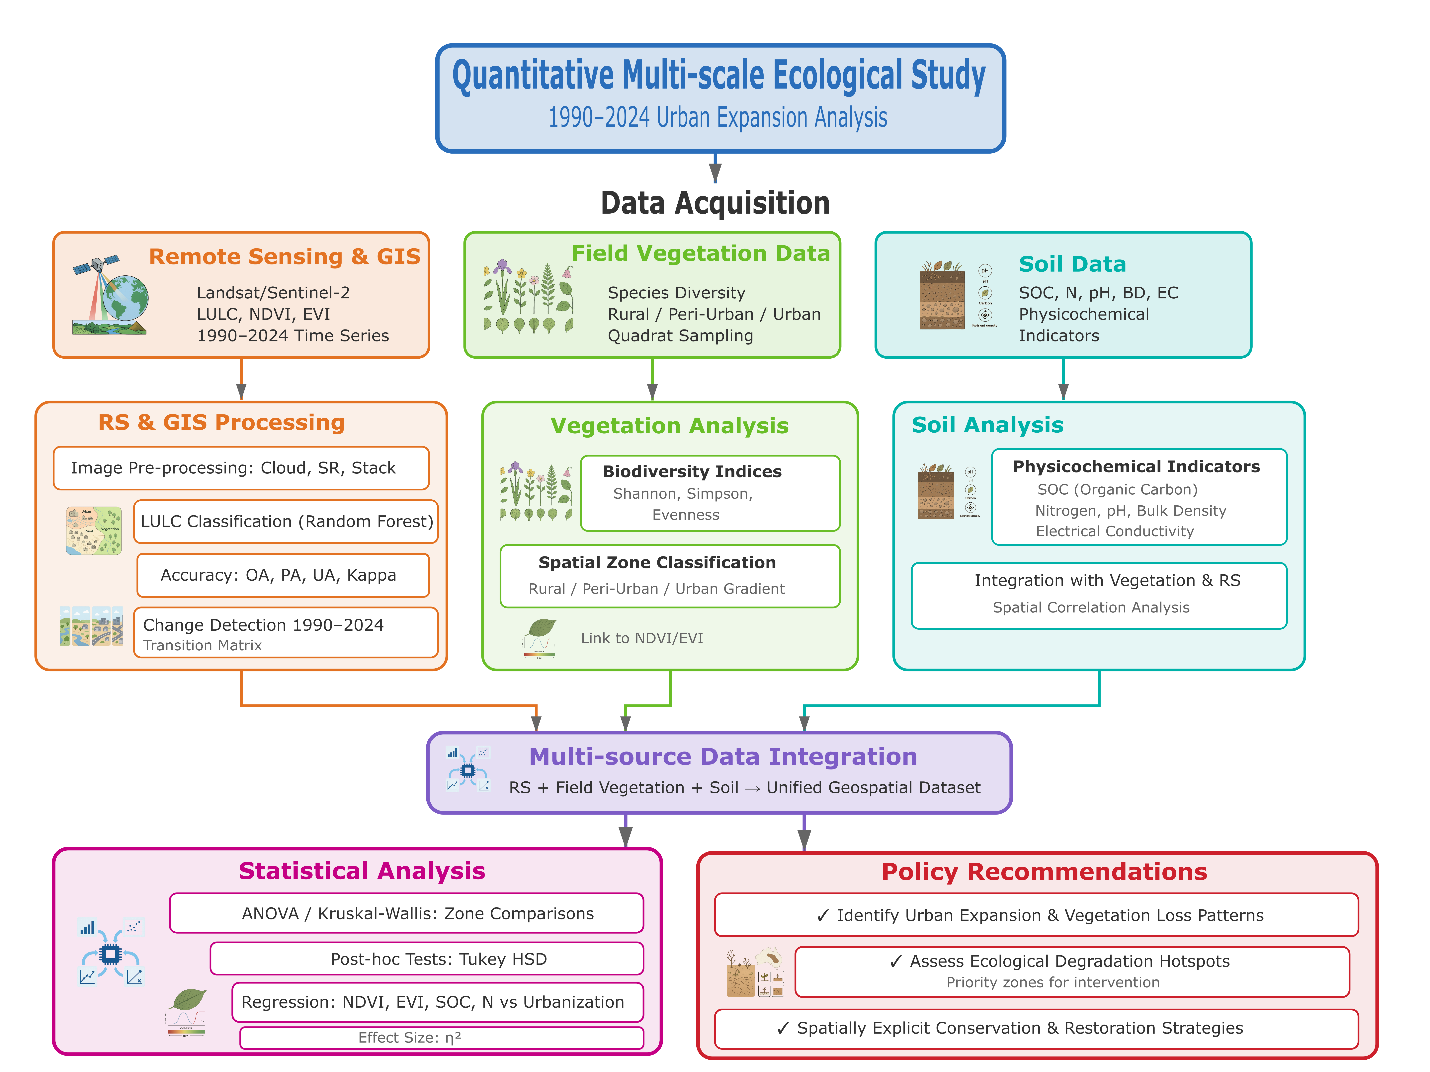
\includegraphics[width=6.5in,height=4.875in]{figures/media/image2.png}

\textbf{Figure 2.1:} Flowchart of Methodological Framework: Author source

{}\textbf{2.2 Study Area}

Benue State, in the north cental of Nigeria, had a land area of 2,882 km² and a population of 4,253,641. The state was divided into twenty-three (23) local government areas. Geographically, Benue State lies within the lower River Benue, with longitude coordinates ranging from 7º 47\textquotesingle{} to 10° 0\textquotesingle{} East and latitude coordinates from 6º 25\textquotesingle{} to 8° 8\textquotesingle{} North (Figure 2.1). The state shares boundaries with five other states: Nasarawa to the north, Taraba to the east, Cross River to the south, Enugu to the southwest, and Kogi State to the west. Additionally, the state shares a common boundary with the Republic of Cameroon to the south-east (Mbah et al. 2016). Benue is characterised by a mix of urban and rural environments, with diverse ecosystems ranging from tropical forests to wetlands and agricultural areas. This study focuses on two cities, Makurdi and Otukpo. Makurdi Local Government Area is situated in the north-eastern part of the State and within the coordinates 7° 00\textquotesingle{} N to 7° 45\textquotesingle{} N latitude and 8° 00\textquotesingle{} E to 8° 32\textquotesingle{} E longitude. The area is drained by several channels, including the River Benue, which bisects the town into north and south banks, and its tributaries, such as Urudu, Demepe, Kereke, Mu, Idye, and Kpege. According to the 1991 and 2006 population censuses, the population of Makurdi was 239,889 and 297,398, respectively. Using a growth rate of 0.03\%, the projected population of Makurdi in 2017 was 517,342. The area has a rapidly growing population of human, with a density of 323 persons per square kilometre. The population is predominantly Tiv-speaking, with other ethnic groups also present. The growth of Makurdi town has put pressure on natural resources within its environs, including wetlands. Makurdi\textquotesingle s climate is characterised by wet and dry seasons. The mean duration of the rainy season is 182 days, with the highest monthly rainfall total of 221 mm recorded in August (Hemba et al. 2017) (see Figure 2.1).
Otukpo is a local government in the Southern Guinea Savannah Zone in north central Nigeria. Otukpo LGA lies on the North of the equator between (the longitude 7° 50\textquotesingle{} and the 8° 15\textquotesingle{} East and the latitude 7° 00\textquotesingle{} and that of 7° 40\textquotesingle). It has a landmass of about 1,385 square kilometres and a population of 266,411 human according to (NPC, 2006) and was projected to be 359,600 people in 2016. The map of Otukpo LGA is shown in Figure 2.2. The general relief of the study area ranges between 83m above sea level and 162 m above mean sea level. The study area is a valley given the area is undulating to gently sloping in the north-south direction. (Ancha et al., 2021) (see Figure 2.2).
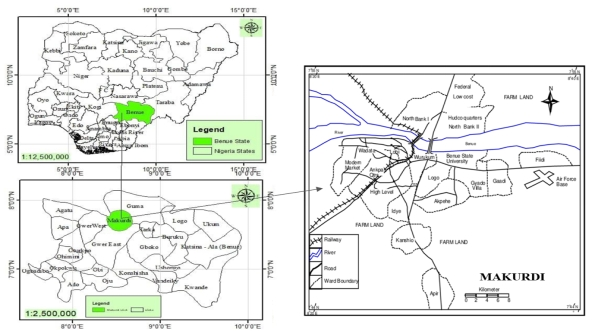
\includegraphics[width=6.19792in,height=3.44792in]{figures/media/image3.jpeg}

\textbf{Figure 2.2:} Map of Makurdi Local Government Area

Source (YAGER, et al. 2024) \& Benue State Ministry for Lands and Survey

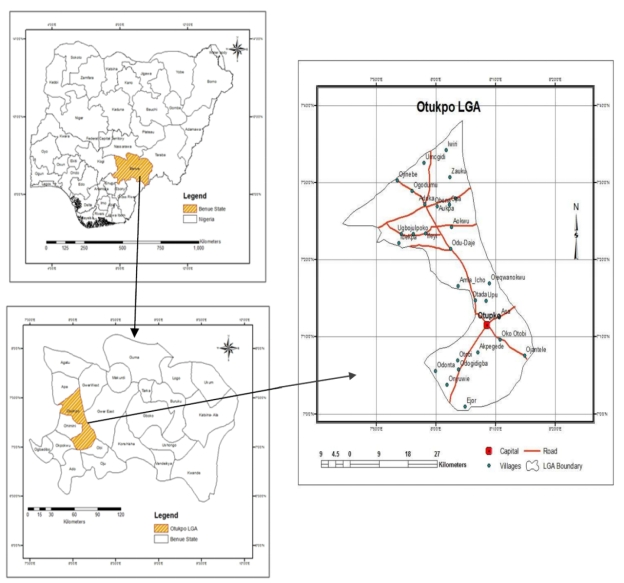
\includegraphics[width=6.5in,height=6.07292in]{figures/media/image4.jpeg}

\textbf{Figure 2.3:} Map of Otukpo Local Government source:(Ancha et al., 2021)

\hypertarget{data-requirements-and-sources}{%
\section{\texorpdfstring{\textbf{2.3 Data Requirements and Sources}}{2.3 Data Requirements and Sources}}\label{data-requirements-and-sources}}

\hypertarget{remote-sensing-data}{%
\section{\texorpdfstring{\textbf{2.3.1 Remote Sensing Data}}{2.3.1 Remote Sensing Data}}\label{remote-sensing-data}}

The study employed temporal satellite imagery and ancillary geospatial datasets necessary for detecting LULC transformations and transitions over time and space, quantifying vegetation condition, and assessing urbanization intensity across the two study locations Makurdi and Otukpo. Landsat TM for the (1990) period, ETM+ for the (2010) period, and the OLI (2024) scenes were obtained for change detection, NDVI, and EVI derivation due to their 30 m spatial resolution and long-term continuity, which makes them suitable for landscape-scale ecological studies. VIIRS Day/Night Band night-time lights imagery was used to represent anthropogenic intensity and built-up expansion through illumination patterns, while WorldPop population density rasters provided high-resolution demographic information to quantify population-driven urbanization pressures these were extracted at the ward level using Appendix 1. In addition, the administrative boundary datasets for wards and LGAs were incorporated to enable spatial disaggregation of results and zonal analyses. All remote sensing derived layers were clipped, standardized, and extracted at both ward level (point sampling) and zonal level (rural, peri-urban, urban) to match the scales of ecological assessment.
\hypertarget{field-plant-data}{%
\section{\texorpdfstring{\textbf{2.3.2 Field Plant Data}}{2.3.2 Field Plant Data}}\label{field-plant-data}}

The Plant data were obtained through a systematic field sampling conducted across the 33 stratified plots samples, resulting in a detailed dataset comprising species inventories, abundance records, and structural attributes for each sampling location within both study regions. To adequately represent the vertical complexity characteristic of tropical ecosystems, vegetation layers---trees, shrubs, and herbs---were documented separately based on site conditions. For every plot, my team of experts observed and documented the geographic coordinates, its elevation, the surrounding land-use characteristics, and other relevant metadata suitable for the study were recorded to ensure precise spatial referencing and seamless integration with remotely sensed datasets. These collected and documented field observations for both locations formed the basis for calculating biodiversity indices, including Shannon, Simpson, and Evenness, and facilitated comparative analysis of species composition along the rural--peri-urban--urban gradient.
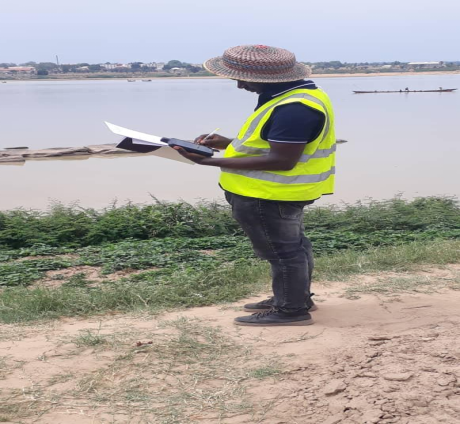
\includegraphics[width=5.57292in,height=5.375in]{figures/media/image5.png}

\textbf{FIG 2.4:} Ground Truth Data Collected During Field Visits on LULC:
Author source

\hypertarget{soil-data}{%
\section{\texorpdfstring{\textbf{2.3.3 Soil Data}}{2.3.3 Soil Data}}\label{soil-data}}

Soil data were obtained using the GEE a cloud computing platform to assess the ecosystem functioning through the following key soil biophysical properties; 1) soil organic carbon (SOC), 2) total nitrogen, 3) bulk density, 4) soil pH, and 5) the cation exchange capacity (CEC), which together provide insight into soil fertility, compaction levels, and overall chemical balance. These soil variables were extracted from globally validated soil datasets suitable for sub-Saharan Africa and spatially matched to the vegetation sampling plots. The soil information was then integrated with field-based vegetation data and remotely sensed variables to evaluate how urbanization influences soil quality and related ecological processes along the rural--peri-urban--urban gradient. The GEE workflow used for extracting the soil variables is provided in Appendix 1.
\hypertarget{land-use-and-land-cover-lulc-analysis}{%
\section{\texorpdfstring{\textbf{2.4 Land-Use and Land-Cover (LULC) Analysis}}{2.4 Land-Use and Land-Cover (LULC) Analysis}}\label{land-use-and-land-cover-lulc-analysis}}

\hypertarget{image-pre-processing}{%
\section{\texorpdfstring{\textbf{2.4.1 Image Pre-Processing}}{2.4.1 Image Pre-Processing}}\label{image-pre-processing}}

All satellite images were pre-processed to ensure radiometric consistency and spatial comparability across the three temporal periods (1990, 2010, 2024). Landsat Surface Reflectance (SR) products generated using LEDAPS for TM/ETM+ and LaSRC for OLI were used, as these datasets provide atmospherically corrected spectral bands suitable for quantitative analysis. Cloud and cloud-shadow contamination were removed using the pixel-level quality assurance (QA) masks embedded in the SR products. After performing the cloud removal on the imageries, the individual spectral bands were combined to form multi-band images for each study year. These images were then clipped to the administrative boundaries of Makurdi and Otukpo Local Government Areas using official shapefiles, ensuring that the analysis was restricted to the study areas only. And to ensure consistency across time and datasets, all imagery were resampled to a uniform 30m spatial resolution, this is to allow a more reliable comparison between years and seamless integration with NDVI, EVI, and land-use classification outputs.
\hypertarget{lulc-classification-using-random-forest}{%
\section{\texorpdfstring{\textbf{2.4.2 LULC Classification Using Random Forest}}{2.4.2 LULC Classification Using Random Forest}}\label{lulc-classification-using-random-forest}}

The LULC mapping was carried out using a supervised classification approach (Random Forest) machine-learning algorithm. This method was selected because of its reliability, strong performance in handling complex, non-linear relationships, and its suitability for heterogeneous tropical environments. The training samples for the classification purpose were compiled from field-collected GPS points, high-resolution Google Earth imagery, and expert visual interpretation of distinct land-cover features across the study areas.
The Random Forest model was implemented using 500 decision trees, with tuning parameters adjusted to achieve a balance between model accuracy and stability. Five major land-cover classes were defined for the purpose of the classification: 1) the vegetation, 2) the built-up areas, 3) the agricultural land, 4) the bare surfaces, and 5) the water bodies. Following classification, a simple post-classification filtering procedure was applied to reduce the salt-and-pepper effect commonly associated with pixel-based classifications. The final land-use and land-cover maps produced for each study year were then visually examined to confirm spatial consistency and ensure that the classification results reasonably reflected ground conditions.
\hypertarget{accuracy-assessment}{%
\section{\texorpdfstring{\textbf{2.4.3 Accuracy Assessment}}{2.4.3 Accuracy Assessment}}\label{accuracy-assessment}}

The accuracy of each LULC map was evaluated through the independent set of validation points versus the classified outputs were compared against reference data (see Appendix 2). Each map was evaluated to acertain the classification performance using Confusion metric. And the overall accuracy, that reflects the proportion of the correctly classified pixels; the Producer's Accuracy, that measured how effectively real-world LULC types were captured by the classification; the User's Accuracy, which indicated the reliability of each mapped class; and the Kappa coefficient, which accounts for agreement beyond random chance were all performed to all the temporal classifications done.
In all, the accuracy measures provided a robust and effective basis for the evaluating of the classifier performance and confirmed the suitability of the Random Forest approach for land-use and land-cover mapping in complex tropical landscapes.
\hypertarget{lulc-change-detection}{%
\section{\texorpdfstring{\textbf{2.4.4 LULC Change Detection}}{2.4.4 LULC Change Detection}}\label{lulc-change-detection}}

The LULC change was analysed by comparing the classified maps for 1990, 2010, and 2024. A transition matrix was used to track how land-cover classes changed over the 34-year period, allowing gains, losses, and areas of persistence to be clearly quantified. From the change detection analysis also known as post classification, key indicators were derived, including the rate of urban expansion reflected by increases in built-up areas, the extent of vegetation loss indicating reductions in natural and semi-natural cover, and shifts in the distribution of agricultural land and bare surfaces.
\hypertarget{plant-diversity-assessment}{%
\section{\texorpdfstring{\textbf{2.5 Plant Diversity Assessment}}{2.5 Plant Diversity Assessment}}\label{plant-diversity-assessment}}

\hypertarget{sampling-design}{%
\section{\texorpdfstring{\textbf{2.5.1 Sampling Design}}{2.5.1 Sampling Design}}\label{sampling-design}}

A stratified field sampling approach was employed and this is to effectively capture plant diversity across the urbanization zone (rural--peri-urban--urban gradient) in Makurdi and Otukpo LGAs. Stratification was based on administrative wards, by enabling a fine-scale ecological assessment that reflects actual settlement patterns and varying levels of urbanization. In the Makurdi LGA, six wards were sampled out of the 11 wards, wherein each ward three plots were sampled, this resulted to a total of 18 plots. Similarly, in Otukpo, five wards were sampled with three plots each, giving 15 plots. In total, 33 field plots (see Appendix 3, 3P1--3P33) were established across the two LGAs to ensure comprehensive and representative vegetation data.
A nested hierarchical plot design was used to capture plant diversity across different vegetation layers. For trees, a 10 m × 10 m quadrat was set up at each plot. Within each tree plot, a 5 m × 5 m subplot was designated for shrubs, and a 1 m × 1 m subplot placed centrally for herbaceous species for consistency purposed. The choosen layout allowed for simultaneous measurement of species composition, density, and abundance across vertical strata. All plant species within the plots were identified in the field using standard botanical guides, and voucher specimens were collected for species that required further verification. Species abundance was recorded for each stratum, and GPS coordinates were logged to support spatial referencing and integration with remote sensing and regression analyses. This sampling framework produced a detailed vegetation dataset suitable for calculating species richness, Shannon-Wiener diversity, Simpson diversity, and species evenness across the urbanization gradient.
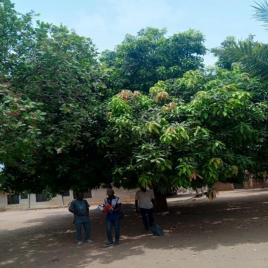
\includegraphics[width=2.79167in,height=2.79167in]{figures/media/image6.png} 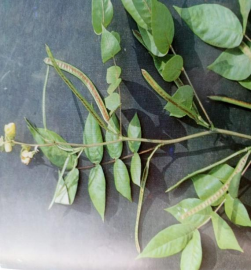
\includegraphics[width=2.625in,height=2.8125in]{figures/media/image7.png}


Mango tree \emph{(Mangifera indica)} Coffee senna \emph{(Senna occidentalis)}


\textbf{FIG 2.5: Field Work on Plants Species Diversity Data Collection:} Author source

\hypertarget{biodiversity-indices-computation}{%
\section{\texorpdfstring{\textbf{2.5.2 Biodiversity Indices Computation}}{2.5.2 Biodiversity Indices Computation}}\label{biodiversity-indices-computation}}

Plant diversity was quantified for each of the 33 plots using three widely applied ecological diversity metrics. These indices provide complementary information on species richness, abundance distribution, and community structure, enabling robust comparison across the urbanization gradient.
Shannon-Wiener Diversity Index (H′)

\[H^{'} = - \sum_{}^{}{p_{i}\ln\left( p_{i} \right)}\]

Where:
\begin{itemize}
\item
  \(p_{i}\)=\(\frac{n_{i}}{N}\)
\item
  \(n_{i}\) = number of individuals of species i
\item
  N = total number of individuals in the plot
\end{itemize}

This index captures both species richness and evenness, with higher values indicating greater diversity and ecological complexity.
Simpson's Diversity Index (1 − D)

\[1 - D = 1 - \sum_{}^{}p_{i}^{2}\]

This index emphasizes species dominance and community balance. Values closer to 1 signify more diverse and less dominated plant communities.
Pielou's Evenness (E)

\[E = \frac{H^{'}}{\ln S}\]

Where:
\begin{itemize}
\item
  S = total number of species recorded in the plot
\end{itemize}

Evenness values close to 1 indicate equitable distribution of individuals across species, reflecting stable and undisturbed vegetation communities.
The computation of these indices provided quantitative measures for evaluating how plant diversity structure responds to increasing levels of urbanization (Solymosi et al. 2019; Xie et al. 2020; Bai et al. 2017).
\hypertarget{statistical-analysis-of-diversity}{%
\section{\texorpdfstring{\textbf{2.5.3 Statistical Analysis of Diversity}}{2.5.3 Statistical Analysis of Diversity}}\label{statistical-analysis-of-diversity}}

\hypertarget{one-way-anova}{%
\section{\texorpdfstring{\textbf{2.5.3.1 One-Way ANOVA}}{2.5.3.1 One-Way ANOVA}}\label{one-way-anova}}

A one-way Analysis of Variance (ANOVA) was applied to test whether plant diversity metrics differed significantly across the three urbanization zones urban, peri-urban, and rural (Ross and Willson 2017). The dependent variables included:
\begin{itemize}
\item
  Shannon-Wiener Diversity Index (H′)
\item
  Simpson's Diversity Index (1 − D)
\item
  Pielou's Evenness (E)
\end{itemize}

Prior to the analysis, the ANOVA assumptions (normality and homogeneity of variances) were verified using Shapiro-Wilk and Levene's tests. Where the assumptions were met, ANOVA was used to determine whether mean diversity values differed among the zones. In the case where the assumptions are violated, the analysis were supported by visual inspection and potential reporting of ANOVA results as supplementary information. A Post-hoc comparisons (Tukey HSD) were conducted where ANOVA yielded significant differences, and this helped in identify specific zone-level contrasts. This statistical approach enabled rigorous assessment of how urbanization intensity influences species diversity and community structure across Makurdi and Otukpo.
\hypertarget{post-hoc-tests}{%
\section{\texorpdfstring{\textbf{2.5.3.2 Post-hoc Tests}}{2.5.3.2 Post-hoc Tests}}\label{post-hoc-tests}}

Where the one-way ANOVA indicated significant differences among the urban, peri-urban, and rural zones, Tukey's Honestly Significant Difference (HSD) test was employed for pairwise comparisons. Tukey HSD identifies which specific pairs of zones differ significantly in terms of:
\begin{itemize}
\item
  Shannon--Wiener Diversity Index (H′)
\item
  Simpson's Diversity Index (1 − D)
\item
  Pielou's Evenness (E)
\end{itemize}

This post-hoc procedure controls for Type I error across multiple comparisons and provides robust inference on the specific effects of urbanization intensity on plant diversity patterns.
\hypertarget{ecosystem-functioning-and-urbanization-impact-modelling}{%
\section{\texorpdfstring{\textbf{2.6 Ecosystem Functioning and Urbanization Impact Modelling}}{2.6 Ecosystem Functioning and Urbanization Impact Modelling}}\label{ecosystem-functioning-and-urbanization-impact-modelling}}

\hypertarget{urbanization-metrics-extraction}{%
\section{\texorpdfstring{\textbf{2.6.1 Urbanization Metrics Extraction}}{2.6.1 Urbanization Metrics Extraction}}\label{urbanization-metrics-extraction}}

Urbanization intensity for each sampled ward was quantified using the 500 m buffer polygons created around field-validated ward centroids (Appendix 4). These buffers were stored as a single asset (WARD\_ZONES\_BUFFER) and served as spatial units for zonal statistics extraction in GEE using Appendix 1. Three primary urbanization metrics were computed for each buffer:
\begin{enumerate}
\def\labelenumi{\arabic{enumi}.}
\item
Built-up Percentage (\% Built-up)
\end{enumerate}

Derived from the ESA WorldCover 2021 land-use map. Pixels classified as ``Built-up (50)'' were extracted and expressed as the mean proportion of built-up area within each buffer.
\begin{enumerate}
\def\labelenumi{\arabic{enumi}.}
\setcounter{enumi}{1}
\item
Night-time Light Intensity (NTL)
\end{enumerate}

Obtained from VIIRS 2024 monthly composites. Mean radiance within each buffer served as a proxy for anthropogenic activity and infrastructure intensity.
\begin{enumerate}
\def\labelenumi{\arabic{enumi}.}
\setcounter{enumi}{2}
\item
Population Density
\end{enumerate}

Extracted from the WorldPop 2020 gridded population dataset. Mean population density within each buffer was used to represent human pressure.
All extracted metrics were exported from GEE into a unified CSV file and standardized using z-scores before regression modelling to ensure comparability and reduce scale effects.
\hypertarget{ecosystem-function-indicators}{%
\section{\texorpdfstring{\textbf{2.6.2 Ecosystem Function Indicators}}{2.6.2 Ecosystem Function Indicators}}\label{ecosystem-function-indicators}}

Ecosystem functioning indicators were derived for each ward buffer using harmonized remote-sensing and soil datasets (Appendix 1). Indicators were computed as buffer-level means and exported as attributes for each ward:
Vegetation Function Indicators

\begin{itemize}
\item
NDVI (Normalized Difference Vegetation Index)
\end{itemize}


Derived from the surface reflectance Landsat 8 (2024) composite using:
\[NDVI = \frac{NIR - RED}{NIR + RED}\]


\begin{itemize}
\item
EVI (Enhanced Vegetation Index)
\end{itemize}


Computed using:
\[EVI = 2.5 \times \frac{NIR - RED}{NIR + 6.RED - 7.5.BLUE + 1}\]


Soil Ecosystem Indicators (from SoilGrids)

\begin{itemize}
\item
  Soil Organic Carbon (SOC)
\item
  Total Nitrogen (N)
\item
  Bulk Density (BD)
\item
  Cation Exchange Capacity (CEC)
\item
  Soil pH
\end{itemize}

These variables reflect soil fertility, physical properties, and chemical status key proxies for ecosystem functioning. All indicators were extracted using GEE's reduceRegions function and exported as a single CSV for analysis (Appendix 5).
{}\textbf{2.6.3 Zone Comparison Statistics}

To evaluate differences in ecosystem functioning across the urban--peri-urban--rural gradient, each ward was categorized into one of the three zones based on pre-field and Google Earth Pro classification (Appendix 4). The following analyses were performed:
\begin{enumerate}
\def\labelenumi{\arabic{enumi}.}
\item
One-way ANOVA
\end{enumerate}

Used to test significant differences among the three zones for:
\begin{itemize}
\item
  NDVI
\item
  EVI
\item
  SOC
\item
  Nitrogen
\item
  Bulk Density
\item
  pH
\item
  CEC
\end{itemize}

\begin{enumerate}
\def\labelenumi{\arabic{enumi}.}
\setcounter{enumi}{1}
\item
Post-hoc Tests
\end{enumerate}

Tukey HSD was applied where ANOVA indicated significant differences.
\begin{enumerate}
\def\labelenumi{\arabic{enumi}.}
\setcounter{enumi}{2}
\item
Effect Size (η²)
\end{enumerate}

Eta squared values were computed to quantify the magnitude of zone effects on ecosystem indicators.
4. Assumptions Checks

\begin{itemize}
\item
  Normality (Shapiro-Wilk and Q-Q plots)
\item
  Homogeneity of variance (Levene's test)
\end{itemize}

This step helps establish whether ecological functioning declines systematically with increasing urbanization.
{}\textbf{2.6.4 Regression Modelling}

A Multiple linear regression was employed to quantify how urban expansion influences plant functioning across the sampled wards. The analysis relied on the integrated ward level dataset containing built-up density, night-time light intensity, population density, and the vegetation response variable. Also, to maintain statistical clarity and avoid model inflation, the regression was restricted to a single vegetation functioning index the NDVI. The decision was guided by the well-established reliability of NDVI as a robust proxy for vegetation productivity, canopy greenness, and photosynthetic condition in heterogeneous tropical landscapes. According to these literatures (Núñez et al. 2011; Luu et al. 2021), NDVI is less susceptible to saturation and background noise than any other greenness index when applied across mixed urban to rural mosaics, making it particularly suitable for any urban ecological evaluation.
NDVI was therefore used as the dependent variable in a single ecological response model, while built-up density, night-time lights, and population density served as the explanatory variables representing the urbanization gradient. The regression structure is expressed as:
~\emph{\hfill\break
}\[NDVI = \beta_{0} + \beta_{1}(Built - up) + \beta_{2}(Lights) + \beta_{3}(Population) + \varepsilon\]

By centering the analysis on a single, theoretically validated indicator, the regression results offer a clearer ecological narrative and a more statistically stable assessment of urbanization impacts.~ To achieve all of these, all statistical analysis were performed in Google Colab Python environment using the following python scripts (Appendix 6, 7 and 8).
{}\textbf{2.7 Policy and Management Recommendations}

The Policies and management recommendations for Makurdi and Otukpo were developed by the absolute synthesization of the major analytical outputs of the study, including LULC change trends, landscape diversity metrics, NDVI variability, soil condition indicators, and regression model relationships between urbanization intensity and ecological variables. The spatial and temporal patterns derived from the LULC analysis provided the researcher with the basis for identifying where urban expansion, vegetation loss, or agricultural conversion is most significant. These were complemented by diversity metrics, which revealed the extent of landscape fragmentation or homogenization across rural, peri-urban, and urban zones. The extraction of both soil and NDVI further highlighted areas experiencing vegetation stress, declining soil quality, or ecological degradation, while the regression models quantified the influence of urbanization on vegetation and soil conditions.
These multiple lines of evidence were integrated systematically to formulate targeted, data-driven policy recommendations. Each of these recommendation were anchored directly to specific findings such as areas showing rapid built-up expansion, high fragmentation, low vegetation vigor, elevated bulk density, or strong regression-based degradation signals. This adopted approach ensured that the final recommendations are not generic but rather spatially explicit, evidence-based, and tailored to the distinct characteristics of rural, peri-urban, and urban environments within both LGAs.
